\section{Resultados}

\begin{table}[!htb]
\begin{center}
\begin{tabular}{|c|c|c|l|c|c|c|c|c|}
\hline
Comb. & Alpha & Beta & Mínimo & Máximo & Promedio & Mediana & Varianza & $Q3-Q1$\\
\hline
1 & 0.1 & 0.9 & 796.066 & 833.597 & 810.658 & 809.587 & 7.866 & 8.669\\
2 & 0.2 & 0.8 & 793.100 & 823.389 & 811.775 & 812.867 & 7.468 & 6.131\\
3 & 0.3 & 0.7 & 797.115 & 830.328 & 811.447 & 810.370 & 7.695 & 7.186\\
4 & 0.4 & 0.6 & 798.210 & 824.965 & 811.827 & 812.077 & 8.061 & 13.158\\
5 & 0.5 & 0.5 & 795.848 & 834.451 & 811.576 & 809.354 & 9.325 & 11.729\\
6 & 0.6 & 0.4 & 790.074 & 828.434 & 808.592 & 809.471 & 8.340 & 10.387\\
7 & 0.7 & 0.3 & 802.024 & 835.707 & 815.194 & 815.560 & 7.863 & 12.762\\
8 & 0.8 & 0.2 & 796.614 & 824.167 & 812.807 & 813.177 & 8.007 & 11.637\\
9 & 0.9 & 0.1 & 800.306 & 832.345 & 811.431 & 811.591 & 8.366 & 11.234\\
\hline
\end{tabular}
\end{center}
\caption{Tabla comparativa del hipervolumen obtenido por }
\label{fig:resumen}
\end{table}

\begin{table}[!htb]
\begin{center}
\begin{tabular}{|l|l|l|l|l|l|l|l|l|l|l|}
\hline
\diagbox[width=5em]{Semilla}{Comb.} & \multicolumn{1}{c|}{1} & \multicolumn{1}{c|}{2} & \multicolumn{1}{c|}{3} & \multicolumn{1}{c|}{4} & \multicolumn{1}{c|}{5} & \multicolumn{1}{c|}{6} & \multicolumn{1}{c|}{7} & \multicolumn{1}{c|}{8} & \multicolumn{1}{c|}{9} \\
\hline
1 & 816.163 & 813.507 & \textbf{830.328} & 819.681 & 809.633 & 810.624 & 813.893 & 815.036 & 816.009\\
\hline
2 & 823.389 & \textbf{823.389} & 808.234 & 814.946 & 818.626 & 811.503 & 818.356 & 820.906 & 811.658\\
\hline
3 & 803.074 & \textbf{793.1} & 818.424 & 818.843 & 807.143 & 819.121 & 821.224 & \textbf{796.614} & 806.735\\
\hline
4 & 815.429 & 809.43 & 807.51 & 815.602 & 823.457 & 812.969 & 807.552 & \textbf{824.167} & 804.891\\
\hline
12 & 805.506 & 814.726 & 806.073 & 799.668 & 809.074 & 797.301 & 815.699 & 809.635 & 803.958\\
\hline
23 & 808.364 & 812.57 & 824.773 & 824.284 & 805.076 & 804.597 & 806.314 & 797.416 & 822.47\\
\hline
34 & 814.076 & 814.076 & 814.076 & 814.866 & \textbf{834.451} & 814.034 & 804.079 & 813.902 & 803.117\\
\hline
123 & 809.967 & 813.501 & 804.392 & 814.114 & 806.192 & 800.59 & 822.557 & 803.449 & 823.071\\
\hline
234 & 811.283 & 814.214 & 814.028 & 800.349 & 804.48 & 800.257 & 815.421 & 823.083 & 802.292\\
\hline
345 & 802.239 & 802.239 & 802.239 & 802.239 & 816.866 & 817.043 & 807.465 & 815.962 & \textbf{800.306}\\
\hline
1234 & \textbf{833.597} & 813.161 & 807.917 & 808.785 & 809.739 & 803.514 & \textbf{835.707} & 809.922 & 806.781\\
\hline
2345 & 804.821 & 804.821 & 804.821 & \textbf{824.965} & 824.757 & 808.321 & 808.022 & 821.664 & 811.523\\
\hline
3456 & 803.778 & 803.778 & 810.044 & 819.471 & 805.744 & \textbf{828.434} & 821.831 & 820.55 & 815.256\\
\hline
12345 & 813.886 & 822.197 & 822.139 & 809.516 & 815.895 & 814.689 & 820.129 & 810.818 & 815.852\\
\hline
23456 & 810.286 & 811.333 & 811.333 & 803.559 & 797.033 & 809.753 & 813.877 & 807.049 & 804.963\\
\hline
34567 & 809.206 & 809.206 & 810.696 & 821.231 & 820.865 & 807.526 & 817.814 & 804.268 & 812.303\\
\hline
123456 & 813.979 & 805.951 & 815.12 & 809.577 & 807.865 & 800.852 & \textbf{802.024} & 819.31 & 801.613\\
\hline
234567 & \textbf{796.066} & 822.695 & 810.726 & 806.603 & 814.256 & 809.188 & 810.132 & 820.479 & 820.964\\
\hline
345678 & 809.082 & 822.64 & \textbf{797.115} & 810.04 & 804.516 & 811.446 & 821.302 & 809.464 & \textbf{832.345}\\
\hline
456789 & 808.965 & 808.965 & 808.965 & \textbf{798.21} & \textbf{795.848} & \textbf{790.074} & 820.48 & 812.452 & 812.526\\
\hline
\end{tabular}
\end{center}
\caption{Hipervolumen obtenido con la instancia Mandl 6:2:8 para distintas semillas y combinaciones de valores de alpha y beta. Valores máximos y mínimos obtenidos aparecen resaltados.}
\label{tab:todosmandl}
\end{table}

\begin{figure}[!htb]
\begin{center}
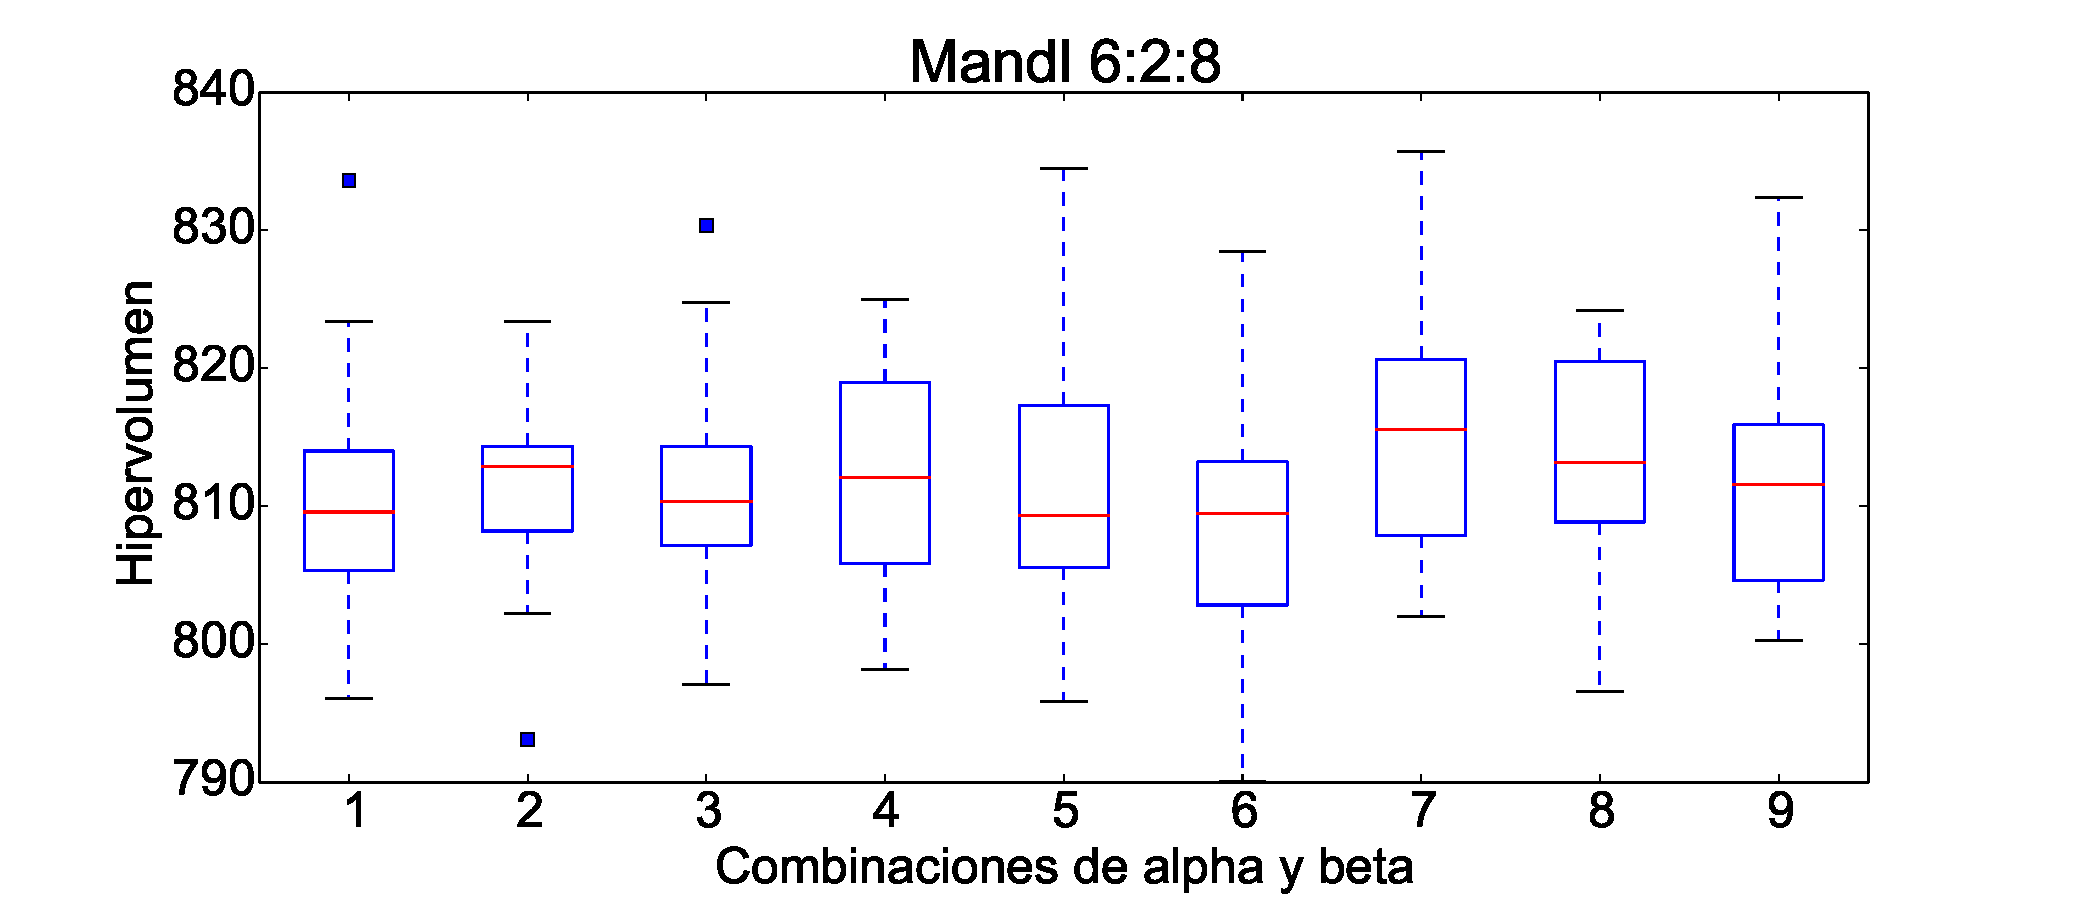
\includegraphics[width=\textwidth]{img/box_plot}
\end{center}
\caption{}
\label{fig:boxplot}
\end{figure}
